
\begin{figure}[h!]
    \centering
    \begin{subfigure}[t]{0.33\textwidth}
    \captionsetup{justification=centering}
        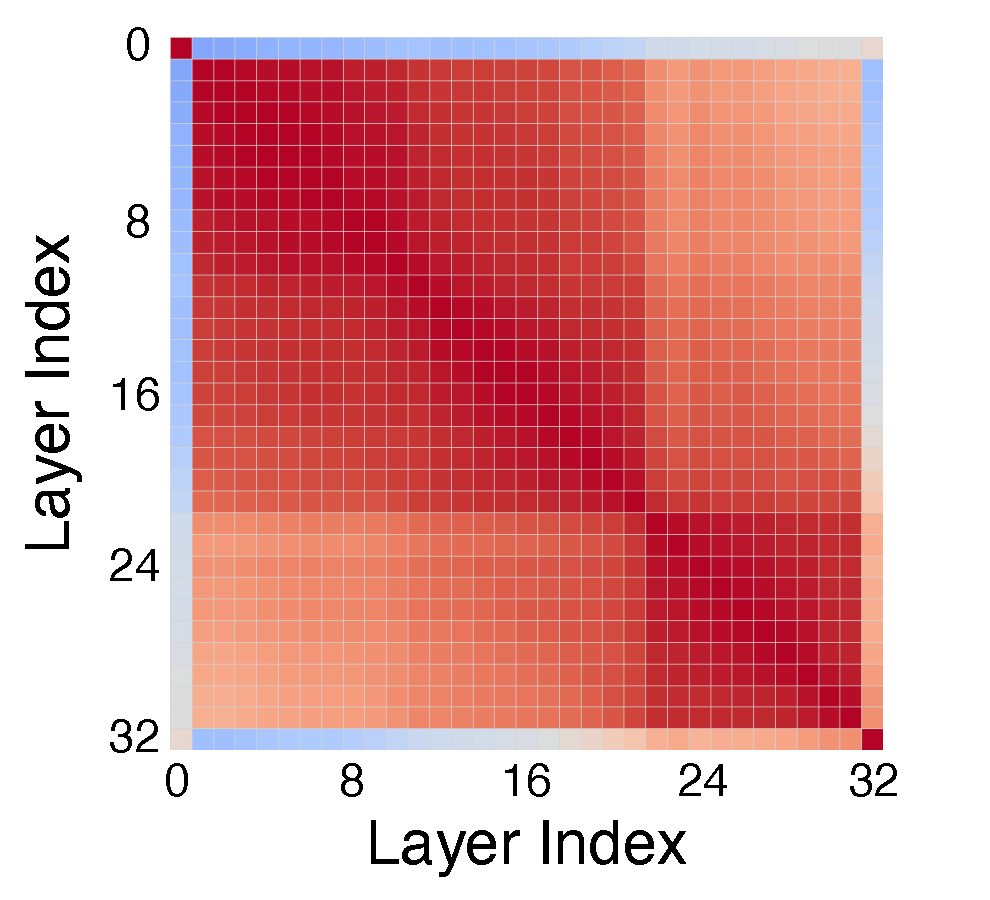
\includegraphics[width=\textwidth]{figs/kv_magnitude/dir_hidden.pdf}
        \subcaption{Hidden states}
    \end{subfigure}
    \centering
    \begin{subfigure}[t]{0.30\textwidth}
    \captionsetup{justification=centering}
        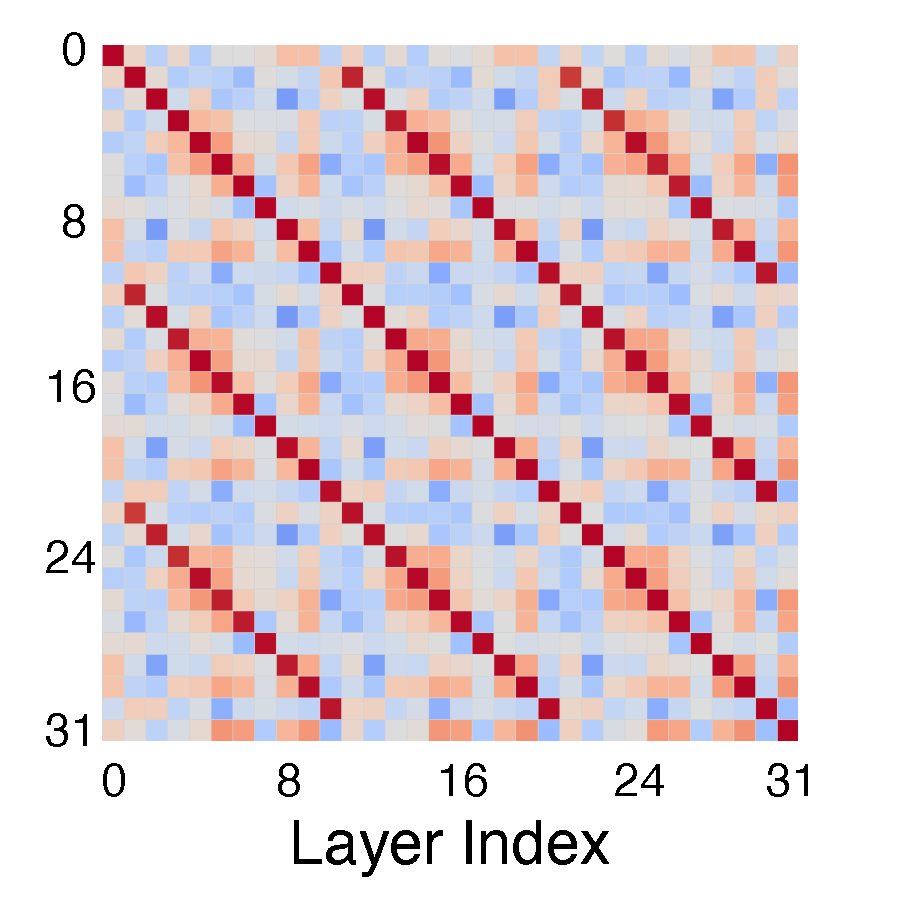
\includegraphics[width=\textwidth]{figs/kv_magnitude/dir_key.pdf}
        \subcaption{Key states}
    \end{subfigure}
    \centering
    \begin{subfigure}[t]{0.33\textwidth}
    \captionsetup{justification=centering}
        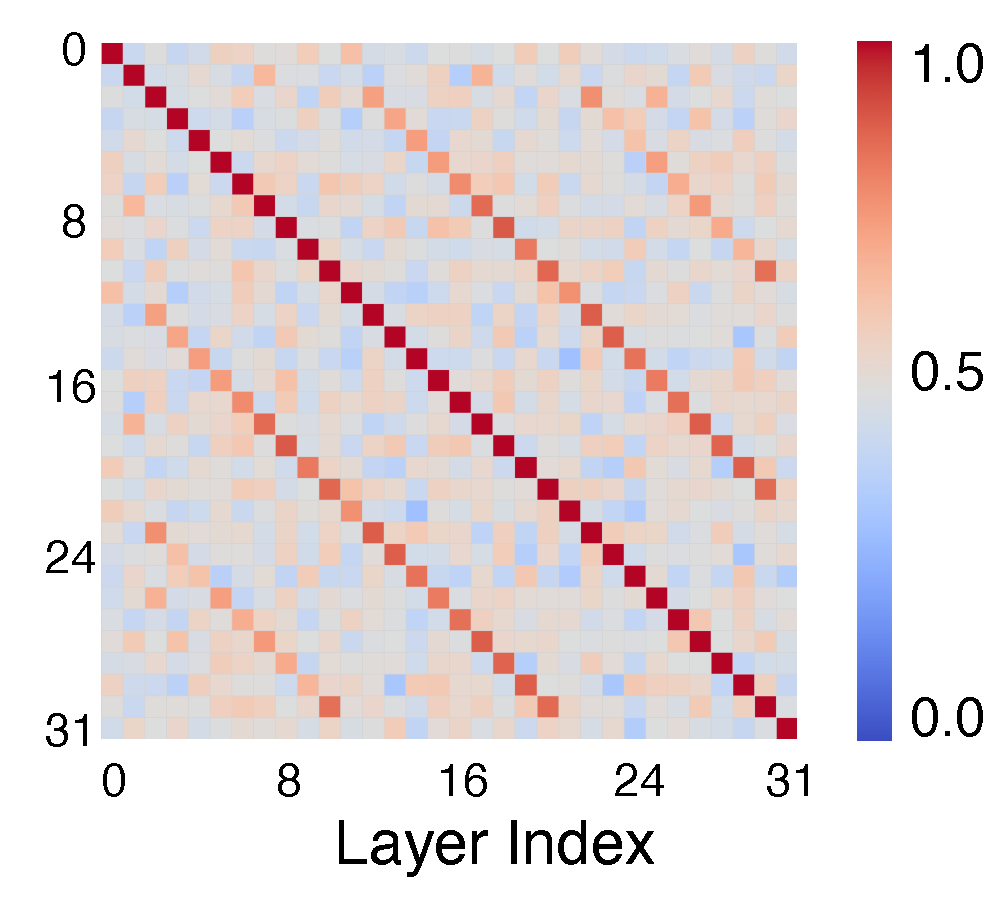
\includegraphics[width=\textwidth]{figs/kv_magnitude/dir_value_cbar.pdf}
        \subcaption{Value states}
    \end{subfigure}
    \caption{ Cosine similarity matrices showing the layer-wise similarity of (a) hidden states, (b) key states, and (c) value states in Recursive Transformer with Middle-Cycle strategy and recursion depth 3. Results are from a 360M parameter model with 32 layers. The hidden states matrix includes the final hidden states after the last layer normalization.
    }
    \label{fig:kv_sharing_dir_app}
\end{figure}